\documentclass{exam}
\usepackage{amssymb}
\usepackage{lipsum} 
\usepackage{graphicx}
\usepackage[
backend=biber
]{biblatex}
\addbibresource{refs.bib}

\usepackage{hyperref}
\hypersetup{
    colorlinks=true,
    linkcolor=blue,
    citecolor=black,
    filecolor=blue,      
    urlcolor=blue,
}

\newcommand\labnr{6}
\newcommand\lab{Lab \labnr\ - Shortest Path Algorithms}

\newcommand\uni{Technical University of Cluj-Napoca}
\newcommand\course{Data Structures \& Algorithms}

\newcommand\lvlez{$\bigstar$}
\newcommand\lvlmed{\lvlez\lvlez}
\newcommand\lvlhard{\lvlmed\lvlez}
\newcommand\lvlvhard{\lvlhard\lvlez}


\pagestyle{headandfoot}
\firstpageheader{}{}{}
\firstpagefootrule
\firstpageheadrule
\firstpagefooter{\sc\uni}{}{\sc\course, Lab \labnr}
\runningheader{\sc\uni}{}{\sc\course, Lab \labnr}
\runningheadrule
\runningfootrule
\runningfooter{}{\thepage}{}

\usepackage{listings}
\usepackage{xcolor}
\usepackage{svg}

\definecolor{codegreen}{rgb}{0,0.6,0}
\definecolor{codegray}{rgb}{0.5,0.5,0.5}
\definecolor{codepurple}{rgb}{0.58,0,0.82}
\definecolor{backcolour}{rgb}{0.95,0.95,0.92}

\lstdefinestyle{mystyle}{
    commentstyle=\color{codegreen},
    keywordstyle=\color{magenta},
    stringstyle=\color{codepurple},
    basicstyle=\ttfamily\footnotesize,
    breakatwhitespace=false,         
    breaklines=true,                 
    captionpos=b,                    
    keepspaces=true,                 
    showspaces=false,                
    showstringspaces=false,
    showtabs=false,                  
    tabsize=2
}
\lstset{style=mystyle}

\begin{document}
\begin{center}
    \vspace*{0cm}
    \bfseries\LARGE
    \lab
    \vspace*{1cm}
\end{center}


\begin{questions}
\question Implement Dijkstra's algorithm using any graph representation you want: \cite{cormen2022introduction}

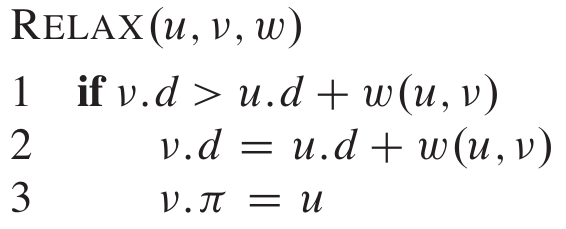
\includegraphics[width=0.25\textwidth]{diagrams/relax.png}

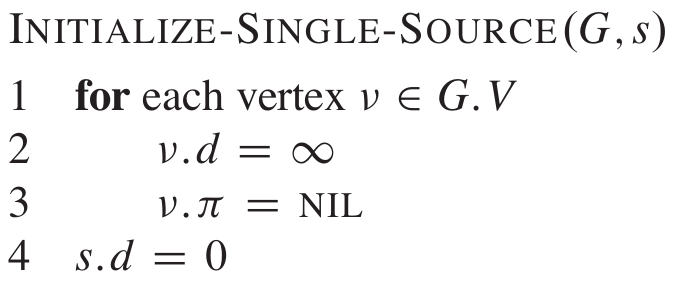
\includegraphics[width=0.3\textwidth]{diagrams/initss.png}

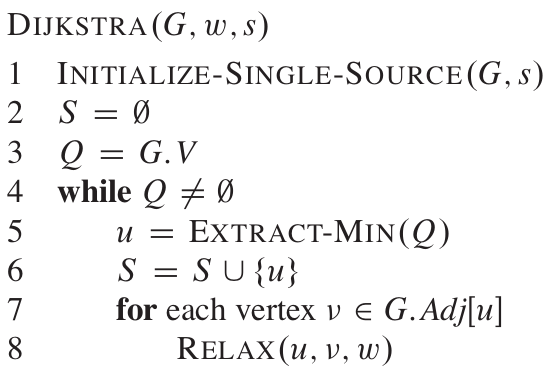
\includegraphics{diagrams/dijkstra.png}


\question Implement the Floyd-Warshall algorithm using any graph representation you want: \cite{cormen2022introduction}

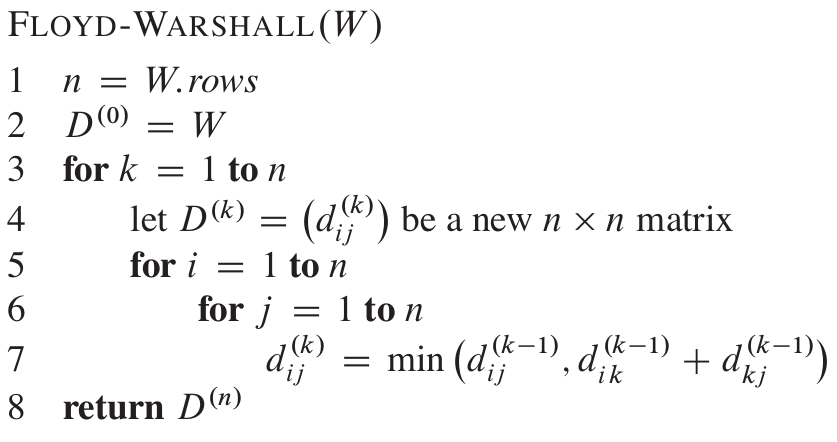
\includegraphics[width=0.4\textwidth]{diagrams/floyd.png}

\question Implement the A* algorithm using any graph representation you want: \cite{astar}

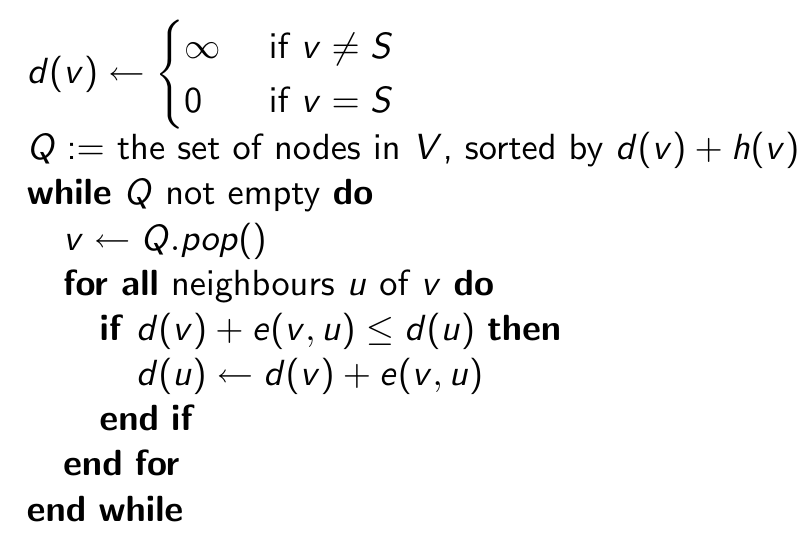
\includegraphics[width=0.4\textwidth]{diagrams/astar.png}

\textbf{Hint:} You can add 2d coordinates to the nodes in the graph and use the Euclidean distance between each node and a destination node as the function $h$


\end{questions}

% \bigskip
\textbf{Note:} Leave a comment with the text PB1, PB2.A.II, ... PB10 above every function that implements the respective lab task. (upper case text, no space between the text and the problem number)

\medskip
\printbibliography
\end{document}
